\chapter{Practical Error correction - Linear codes}
\section{Description, Encoding and Decoding complexity}
Shannon's channel coding theorem provides the limits to what we can do to recover a message that passes through a noisy channel. From the practical point of view, they are not so useful in finding the actual codes and algorithms to perform error correction. They set an important  asymptotic limit on the rate at which we could encode and decode, given the current channel conditions. In practice, finding good codes is a much more extensive area of research, with its own mathematical challenges. In a sense, once the main features of what constitutes a good code are studied, designing them for the problem at hand becomes more of an art. There are three main complexities arising in practical error correction.
\begin{itemize}
	\item Description Complexity: a code can be described by a certain number of parameters. It will become clear, that as in the original Shannon Theorem proof, there exist families of codes that behave similarily and the that can be described with very few parameters. Practical codes have a specific rate of encoding and decoding, meaning that they will achieve a certain portion of the optimal rate (Shannon capacity). The finite size of these codes and the fact that we will constrain the space in which we try to find them (in order to easily design them) will give us a penalty in terms of the actual Capacity up to which they will be able to correct errors well. This is called the capacity gap.
	\item Encoding Complexity: The encoder provides the amount of redundant information needed to be able to correct messages, even in the presence of noise. Although in general the procedure is very similar for a large part of the codes families, it is still an engineering problem to get to the optimal encoding throughput, meaning design fast and reliable encoders.
	\item Decoding Complexity: the decoding algorithm, as we will see, is one that cannot be solved optimally in polynomial time. It is crucial then, to struck the right balance between fast and accurate decoders. While in principle in the asymptotic limit the channel coding problem is one that can be solved (below the channel capacity) or not (above it), in practice, the decoder is a finite processor and might fail even below the capacity, increasing the capacity gap.
\end{itemize}

The main focus of classical and modern coding theory is then to find codes that have a high correction capability, while beign fast and simple to implement. In almost all circumstances obtaining a code that fulfills any of these requirements and strict optimality (in the sense of Shannon theorem) is bound to fail. Still, there is a large class of modern codes that can reach extremely good performance and still be able to work very close to the Shannon limit.

Out of all possible codes, linear codes have the simplest algebraic structure possible. This feature makes them and their performance easy to study. Moreover, the implementation of fast and simple encoders and decoders is possible. They were studied since the inception of information theory. Let's introduce them with a simple example that can catch many of their basic features and then we will generalize their definition and state some important results.

\section{A first example: Hamming Codes}
Hamming codes were invented in the 50s and have been used since then even if they are not as efficient as more modern codes. They are simple, but far from trivial, which makes them the perfect playground, as they show all the basic features of linear codes.

Let's start with the task of sending m bits called the message bits, through a noisy channel. We will denote them as $b_1, \dots, b_m$. We want to add a number of other bits, called parity bits $(p_1, \dots, p_k)$ in such a way that a certain number of equations involving both the message and parity bits are satisfied. Those equations, the parity check equations, are (linear) constraints on the choice of parity bits for each possible set of message bits, as they enforce the overall parity of the bits involved.

Those parity check equations make sure that it is possible, upon their inspection on the received message, to know if there is a certain amount of bits that contain errors. In certain cases we could also know exactly where. This would allow us to correct them.

The Hamming code $\mathcal{H}(n, k, d)$ is one of those codes. We denote $n$ the \textbf{code length}, $k$ the number of message bits, and $d$ the \text{minimum distance}.
Thus, this code has a \textbf{code rate} of $\frac{k}{n}$.

To understand intuitively how this code works let's draw the following Venn diagram:
\def\firstcircle{(90:1.75cm) circle (2.5cm)}
\def\secondcircle{(210:1.75cm) circle (2.5cm)}
\def\thirdcircle{(330:1.75cm) circle (2.5cm)}
\begin{center}
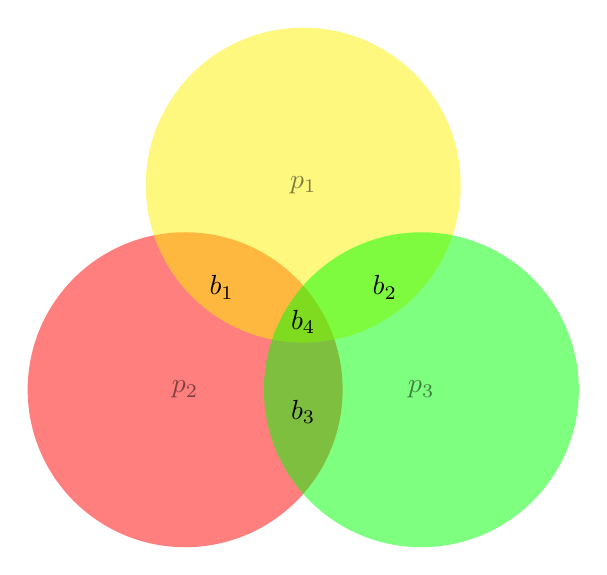
\begin{tikzpicture}[thick,
set/.style = {circle,
	minimum size = 4cm,
	fill=black!30,
opacity=0.5}]

\node (A) [set, fill=red] {$p_2$};
\node (B) at (60:3cm) [set, fill=yellow] {$p_1$};
\node (C) at (0:3cm) [set, fill=green] {$p_3$};

\node at (barycentric cs:A=1,B=1) [left] {$b_1$};
\node at (barycentric cs:A=1,C=1) [below] {$b_3$};
\node at (barycentric cs:B=1,C=1) [right] {$b_2$};
\node at (barycentric cs:A=1,B=1,C=1) [] {$b_4$};
\label{fig:hammingvenn}
\end{tikzpicture}
\end{center}

The three circles are the three parity check equations. The sum of the bits in each circle needs to be zero. This can be written explicitly as the system:

\begin{equation}
	\begin{cases}
		b_1 + b_3 + b_4 +p_1 = 0 \\
		b_1 + b_2 + b_4 +p_2 = 0 \\
		b_2 + b_3 + b_4 +p_3 = 0
	\end{cases}
	\label{eq:hammingsys}
\end{equation}

\begin{example}[Exercise]
Show that as the three parity bits cover the message bits as in the Venn diagram above, this code is capable of correcting one error and detect up to two errors.
\end{example}

Given $x \in \mathbb{F}^3_2 $, we can write the system \ref{eq:hammingsys} as a matrix equation
\begin{equation}
Hx = 0,
\end{equation}
where H is the parity check matrix:
\begin{equation}
H = \left[\begin{matrix}
1 & 0 & 1 & 1 & 1 & 0 & 0 \\
1 & 1 & 0 & 1 & 0 & 1 & 0 \\
0 & 1 & 1 & 1 & 0 & 0 & 1
\end{matrix} \right]
\end{equation}

The parity check matrix is one way in which we can describe completely the error correction scheme. The description complexity problem then amounts to find ways to simplify the structure of this matrix without affecting its correction performances.


We can generalize this construction to an arbitrary number of message bits (called systematic bits). In general, if the code has a number of systematic bits (the dimension of the code) $s$ then its order is $|\mathcal{C}| = 2^{s}$, the number of valid codewords. The Humming code will have $ 2^k -1 $ parity bits equations, for $k$ parity bits. Then the relation between systematic and parity bits is in the dimension of the code: $s = 2^{k} - k - 1$.

\begin{example}[Exercise: General Hamming codes]
	Prove the previous statements.
	[Hints:] How many different subsets of different parity check equations can you build from the whole set of parity check eqs?
\end{example}

The Humming codes can also be just seen as the ones with a H matrix whose columns are all the possible set of $n = 2^k-1$ binary numbers of $k$ bits (apart from the zero element).


Let's dive into how the error correction works and see if we can identify some general features.

\begin{itemize}
	\item Note that our messages will be in $\mathbb{F}^4$ and we will encode them adding three bits to $\mathbb{F}^7$. This map is injective, but not surjective, i.e if two messages are different they will be mapped to different codewords, but some codewords are valid, they come from a message, some are not valid. This is in line with our discussion about minimal distance and packing spheres.

	Out of the $2^7=128$ possible codewords, the valid ones are only $2^4=16$. We can list the 16 valid codewords corresponding to the 16 possible messages.

	\item The codewords set is divided into $2^3$ equivalence classes of $2^4$ elements each. One of these classes is the valid codewords class. The matrix H maps each codeword into a element of $\mathbb{F}^3$ called syndrome. They indicate the equivalence class, with the zero syndrome being the fact the check equations are satisfied, i.e the codeword is valid.
	\item in the specific basis in which we wrote H (yes, we are talking about linear codes so all the sets involved are linear spaces, we will see this!), $c$ is the encoded message sent and $\tilde{c}$ is the received codeword and we assume that it contains one error in the $5-th$ bit, then:
	\begin{equation}
	\begin{split}
	\tilde{c} &= c + e_5, \\
	e_i &= (0, 0, 0, 0, 1, 0, 0), \\
	Hc &= He_5 = (1, 0, 1),
	\end{split}
	\end{equation}
which incidentally is 5 in binary code.

Each code (valid and not valid) has a certain distance from the other measured by the amount of bit flips that are needed to transform one into the other, this is called the Humming distance. 

From the fact that the parity check equation cannot be solved for weight one or two codewords, due to the fact that the columns of the H matrix are linearly independent pairwise, but they are dependent in groups of three, we can infer that the minimum distance is 3, and the code can decode up to 1 error.

 \item \textbf{The generator matrix}. The previously mentioned map that encodes the messages into valid codewords is called G. It has the same information as the H but it can more directly seen as encoding map, if $x \in \mathbb{F}^4$, then $c \in \mathbb{F}^7$ is the corresponding codeword iff:
 \begin{equation}
	 x G^\dagger=c
 \end{equation}
(check: the values of c are the least significant bit of humming distance of the resulting bitwise AND of rows and columns)
\end{itemize}
G can be obtained from H, we will see how in th following.


\section{Tanner Graphs - intro}
The H matrix contains all the information about the error correction code and it can, in principle, be altered without changing the final code. In particular, whenever we perform a permutation of the rows or columns the code remains the same. Even a linear combination of its rows generates a code that does not alter the structure of the code itself. The entire structure of families of codes with similar performances is indeed conveyed not by where the actual ones in the H matrix are but by their number and distribution.

The best representation of the H matrix, being a matrix of zeros and ones is a bipartite graph, called Tanner Graph where the nodes can be divided into variable nodes $V_n$ corresponding to the n input codeword bits and the check nodes $C_k$ corresponding to the check equations. The edges connecting the variable and check nodes are a graphical representations of the parity check equations. For the Humming Code $\mathcal{H}(7,4,3)$ described so far this graph is the one depicted in fig.\ref{fig:TannerHumming}

\begin{figure}[h]
	\begin{center}
		\begin{tikzpicture}[auto]
		\node [pinstyle] (v1) {$v_1$};
		\node [pinstyle, below of = v1] (v2) {$v_2$};
		\node [pinstyle, below of = v2] (v3) {$v_3$};
		\node [pinstyle, below of = v3] (v4) {$v_4$};
		\node [pinstyle, below of = v4] (v5) {$v_5$};
		\node [pinstyle, below of = v5] (v6) {$v_6$};
		\node [pinstyle, below of = v6] (v7) {$v_7$};

		\node [pinstyle, right of=v2, node distance=3cm] (c1) {$c_1$};
		\node [pinstyle, right of=v4, node distance=3cm] (c2) {$c_1$};
		\node [pinstyle, right of=v6, node distance=3cm] (c3) {$c_1$};


		\draw [->] (v1) -- node[name=u] {} (c1);
		\draw [->] (v3) -- node[name=u] {} (c1);
		\draw [->] (v5) -- node[name=u] {} (c1);
		\draw [->] (v7) -- node[name=u] {} (c1);
		\draw [->] (v2) -- node[name=u] {} (c2);
		\draw [->] (v3) -- node[name=u] {} (c2);
		\draw [->] (v6) -- node[name=u] {} (c2);
		\draw [->] (v7) -- node[name=u] {} (c2);
		\draw [->] (v4) -- node[name=u] {} (c3);
		\draw [->] (v5) -- node[name=u] {} (c3);
		\draw [->] (v6) -- node[name=u] {} (c3);
		\draw [->] (v7) -- node[name=u] {} (c3);

		\end{tikzpicture}
	\end{center}
	\caption{The tanner graph of $\mathcal{H}(7,4,3)$}
	\label{fig:TannerHumming}
	\end{figure}

The tanner graph for this specific code has a regular pattern in the check nodes but an irregular one on the variables: each check node has the same degree, but this is not true for variable nodes.We will see this thing in more detail when we generalize these concepts.

\section{General theory of linear codes}

\begin{definition}[Linear code]
	A linear code of length $n$ and dimension $k$ is a linear subspace $C$ with dimension $k$ of the vector space $\mathbb {F}_{q}^{n}$ where $\mathbb {F}_{q}$ is the finite field with $q$ elements.
	The vectors in C are called codewords. The size of a code is the number of codewords and equals $q^k$.
\end{definition}

\begin{definition}[Weight and Distance]
	The weight of a codeword is the number of its non zero element.
	The Humming distance between two codewords is the number of elements in which they differ.
\end{definition}

As we already mentioned a code with codewords of length $n$, dimension $k$ and minimum distance d is denoted as $[n,k,d]$

\begin{definition}[Generator and check matrices]
	As a linear subspace of $\mathbb{F}_{q}^{n}$, the entire code C (which may be very large) may be represented as the span of a set of k codewords (known as a basis in linear algebra). These basis codewords are often collated in the rows of a matrix G known as a \textbf{generating matrix} for the code C. When G has the block matrix form $G=[I_{k}|P]$, where $I_{k}$ denotes the $k\times k$ identity matrix and P is some $k \times (n-k)$ matrix, \textbf{then we say G is in standard form}.

	A matrix H representing a linear function
	\begin{equation}
	H :\mathbb {F}_{q}^{n} \to \mathbb {F}_{q}^{n-k},
	\end{equation}
	whose kernel, $\ker H = \{x \in \mathbb{F}^n_q: H x^T = 0\}$  is C is called a check matrix of C (or sometimes a \textbf{parity check matrix}).

	If C is a code with a generating matrix G in standard form, $G=[I_{k}|P]$, then $H=[-P^{T}|I_{n-k}]$ is a check matrix for C. This form is also called \textbf{systematic}. The code generated by H is called the \textbf{dual code} of C. It can be verified that G is a $k\times n$ matrix, while H is a $(n-k)\times n$ matrix.
\end{definition}

\begin{info}[Syndrome, exact sequences and equivalence classes]
The generating matrix maps our systematic (message bits) in $\mathbb{F}_{q}^{k}$ into a subspace of all possible codewords of length n, $\mathbb{F}_{q}^{n}$  and it is an injection. The H matrix maps $\mathbb{F}_{q}^{n}$ into $\mathbb{F}_{q}^{n-k}$ and it is a surjective map whose kernel is the image of G, namely the linear codes seen so far form the exact sequence:

\begin{equation}
	0 \rightarrow \mathbb{F}_{q}^{k} \xrightarrow{G} \mathbb{F}_{q}^{n} \xrightarrow{H} \mathbb{F}_{q}^{n-k} \longrightarrow 0
\end{equation}
The sequence is called exact when the image of the previous map is the kernel of the following, as in this case, $im(G) = \ker H$. Then the following is true:
\begin{itemize}
	\item G and H are such that GH = 0.
	\item There exist the following bijections: $\mathbb{F}_{q}^{n - k} \cong \mathbb{F}_{q}^{n} / im(G) \cong \mathbb{F}_{q}^{n} / \ker H$,
	\item in turn those bijections mean that the following equivalence classes can be build and they completely separate the codeword space $\mathbb{F}_{q}^{n}$:

	two different codewords $y, y\prime \in \mathbb{F}_{q}^{n}$ that differ by a valid codeword $Gx \in im(G)$, namely $y\prime = y + Gx$ for some $x\in \mathbb{F}_{q}^{k}$ are mapped to the same syndrome by H and so they are in the same equivalence class.
\end{itemize}

\end{info}

The definition of $G$ and $H$ clearly provide an algebraic way to construct one from the other. In their standard form $G$ is lower triangular and $H$ is upper triangular. Using standard LU decomposition (back and forward substitution) one can write them in the standard form and then generate the other.

\begin{info}[A note on duality]
	As we mentioned, the null space of H is actually the code C (the null space is indeed a linear subspace of the full $\mathbb{F}^n$). From the fundamental theorem of algebra (rank-nullity theorem) the full space can be divided into the null space and the image of $H$. The sum is direct, meaning that the elements are orthogonal to each other with respect to an inner product. Whenever there is an orthogonal decomposition of this type the subspaces are called dual to each other. I this case though, even if there exists a productof this kind, it is not, stricly, an inner product.
\end{info}

\begin{theorem}
	In a linear code, the minimum distance between a code word $c_0$  and any other c does not depend on the codeword $c_0$. This means that the minimum distance for the whole code C is the same as the minimum weight codeword's weight
\end{theorem}
\begin{proof}
	Very easy using just linearity. \textcolor{red}{Fill in the details}.
\end{proof}

\begin{theorem}
The distance d of a linear code C also equals the minimum number of linearly dependent columns of the check matrix H.
\end{theorem}
\begin{proof}
	\textcolor{red}{Fill in the details}
\end{proof}

\begin{example}[Exercise]
	Generalize Humming Codes to any n. (hint: the minimum distance is always 3)
\end{example}

\section{MAP decoding for linear codes over BSC}

For linear codes the MAP decoder over BSC is translated to a more algebraic formulation.

\begin{eqnarray}
	x^{ML} &=& \text{argmax}_{x \in C} P_{X|Y}(x|y) \\
	&=& \text{argmax}_{x: Hx^T=0} P_{X|Y}(x|y) \\
	&=& \text{argmax}_{x: Hx^T=0} \epsilon^{d(x,y)}(1-\epsilon)^{n-d(x,y)} \\
	&=& \text{argmax}_{x: Hx^T=0} d(x, y) \\
	&=& \text{argmax}_{x: Hx^T=0} w(x + y) \\
	&=& \text{argmax}_{x: He^T=s^T} w(e) \\
\end{eqnarray}

\section{Description, Encoding and Decoding complexity analysis}
The description complexity of an error correction code can be measured by the maximum amount of degrees of freedom of their respective $H$ and $G$ matrices.
Given that the Generator matrix has dimension $(k, n)$ and the $H$ matrix has dimension $((1-k), n)$, if we don't assume any structure on those matrices and keep the rate $R$ fixed, the description complexity is:
\begin{eqnarray}
	\min\{Rn^2, (1-R)n^2\}
\end{eqnarray}

We will see that this complexity can be greatly simplified assuming a certain structure on the $H$ matrix.

The Encoding complexity is given by the number of operations needed for the encoding task. Given the simple algorithm of solving the encoding equation through the $G$ matrix, this is in general of order $\mathbf{O}(n^2)$. Even in this case it has been proven by Richardson and Urbanke that in many cases the $\mathbf{O}(n^2)$ part is  either highly suppressed or not present altogether, leaving only a complexity of $\mathbf{O}(n)$ operations.

The Decoding complexity as stated in the MAP decoding formula is a lot trickier. This problem is of type NP-complete. These are a class of problems that can be solved by a non-determininstic Turing machine in polynomial time. This is likely to mean that there is no efficient algorithm that can solve the problem in polynomial time.

The fact that this problem is hard does not mean that we cannot achieve good performances with sub-optimal codes and decoding algorithms. First, we need to have in mind that both the code choice and the decoding algorithm have an important role in deciding if we can achieve capacity (be very close to it with probability of error that goes to zero if N becomes large). Actually the proof of Shannon theorem is actually done using a suboptimal decoder!

The decoders that we are going to use are all iterative and we hope to get a good understanding of their convergence properties.

Given a channel characterized by a parameter $\epsilon$ and a channel capacity that depends on it $C(\epsilon)$, a sub-optimal decoder will show a performance curve like the one in fig. \ref{fig:decoder_perf}. The parameter $\epsilon^{BP}$ is called the \textbf{threshold} and acts as an actual capacity that the decoder can achieve with a gap $\delta$ to the true capacity $C(\epsilon)$. This is a typical performance of an error correction code under some decoder that achieves capacity. The different lines correspond to increasing codelength $n$. We can see two different region. The flat one is called \textbf{Error Floor} region. For parameters distant from capacity there are still residual failures (error probability bounded from zero). The vertical or so called \textbf{Waterfall} region is the one where the probability of error falls-off exponentially in the blocklength.

\begin{figure}
	\begin{center}
		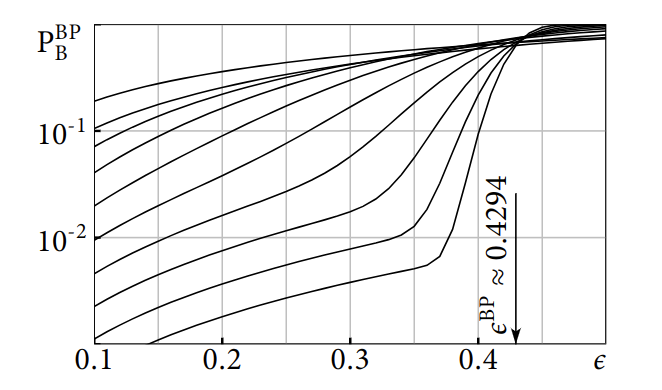
\includegraphics{performances.png} \label{fig:decoder_perf}
		\caption{Performance of decoder}
	\end{center}
\end{figure}
\section{Regular vs irregular Codes}
The Tanner graph picture makes it simple to visualize the connections between variables and check equations. If all the variable nodes have the same number of edges connected to them and so do the check nodes the code is called \textbf{regular}. Any code as a tanner graph can be the seen as having sockets attached to each node. Each socket have a number of edges facing the rest of the graph and the sockets are labelled by the number of edges they provide. See picture \ref{fig:TannerRegular} for an example.

\begin{figure}[h]
	\begin{center}
		\begin{tikzpicture}[auto]
		\node [pinstyle] (v1) {$v_1$};
		\node [socket, right of = v1, node distance=1cm] (vs1) {};
		 		\node [pinstyle, right of = vs1] (v1_b) {};
		 		\node [pinstyle, above of =  v1_b, node distance=0.5cm] (v1_a) {};
		 		\node [pinstyle, below of = v1_b, node distance=0.5cm] (v1_c) {};
		\draw [-] (v1) -- node[name=u] {} (vs1);
			\draw [-] (vs1) -- node[name=u] {} (v1_a);
			\draw [-] (vs1) -- node[name=u] {} (v1_b);
			\draw [-] (vs1) -- node[name=u] {} (v1_c);

		\node [pinstyle, below of = v1, node distance=1cm] (v2){};
		\node [pinstyle, below of = v2	, node distance=2cm] (v4) {$\vdots$};
		\node [pinstyle, below of = v4, node distance=2cm] (v6) {};

		\node [pinstyle, below of = v6, node distance=1cm] (vn) {$v_n$};
		\node [socket, right of = vn, node distance=1cm] (vs1) {};
		\node [pinstyle, right of = vs1] (v1_b) {};
		\node [pinstyle, above of =  v1_b, node distance=0.5cm] (v1_a) {};
		\node [pinstyle, below of = v1_b, node distance=0.5cm] (v1_c) {};
		\draw [-] (vn) -- node[name=u] {} (vs1);
		\draw [-] (vs1) -- node[name=u] {} (v1_a);
		\draw [-] (vs1) -- node[name=u] {} (v1_b);
		\draw [-] (vs1) -- node[name=u] {} (v1_c);


		\node [pinstyle, right of=v2, node distance=6cm] (c1) {$c_1$};
			\node [socket, left of = c1, node distance=1cm] (cs1) {};
 		\node [pinstyle, left of = cs1] (c1_b) {};
 		\node [pinstyle, above of =  c1_b, node distance=0.5cm] (c1_a) {};
 		\node [pinstyle, below of = c1_b, node distance=0.5cm] (c1_c) {};
 		\draw [-] (c1) -- node[name=u] {} (cs1);
 		\draw [-] (cs1) -- node[name=u] {} (c1_a);
 		\draw [-] (cs1) -- node[name=u] {} (c1_b);
 		\draw [-] (cs1) -- node[name=u] {} (c1_c);

		\node [pinstyle, right of=v4, node distance=6cm] (c2) {$\vdots$};
		\node [pinstyle, right of=v6, node distance=6cm] (c3) {$c_{n-k}$};
			\node [socket, left of = c3, node distance=1cm] (csn) {};
			\node [pinstyle, left of = csn] (c1_b) {};
			\node [pinstyle, above of =  c1_b, node distance=0.5cm] (c1_a) {};
			\node [pinstyle, below of = c1_b, node distance=0.5cm] (c1_c) {};

			\draw [-] (csn) -- node[name=u] {} (c1_a);
			\draw [-] (csn) -- node[name=u] {} (c1_b);
			\draw [-] (csn) -- node[name=u] {} (c1_c);

		\end{tikzpicture}
	\end{center}
	\caption{The tanner graph of a regular code}
	\label{fig:TannerRegular}
\end{figure}
Codes will not be considered as a single entity but as a family with the same degree distribution as we saw before. A family (or \textbf{ ensamble}) is then labelled by two numbers corresponding to the degree of each variable and check node respectively, $l$ and $r$.

This parametrization through the nodes degrees $l$, $r$ is a very useful one. To get an idea, one can think about the fact that once the sockets are fixed you can connect the variable and check nodes in only a certain amount of ways. There is a constraint such that you actually are able to use up all edges form all sockets without leftovers. The constraint is very simple you count all the edges involved in the graph from the variable perspective, i.e. $nl$ and all the edges involved from the check perspective $kr$. The number of edges in the graph e is the same and constant so:
\begin{equation}
	nl = kr
\label{eq:edge_constraint_reg}
\end{equation}

The code rate can now be reparametrized by these two numbers and leave the total number of variables independent. So the families of codes are ensambles with a fixed R and variable n.
Using eq. \ref{eq:edge_constraint_reg}
\begin{equation}
	R = \frac{n-k}{n} = 1 -\frac{l}{r}
\end{equation}

\section{LDPC Codes}
The most promising codes in terms of performance are the so called LDPC or Low density parity check codes. They were invented by Gallager in the sixties, but they were rediscovered and analyzed in full only in the late 1990s and 2000s. They are linear codes but with one key characteristic. The H matrix describing them is very sparse. Usually, a code is described in terms of the degree distribution of the corresponding Tanner graph. To start with, we describe a regular $(l,r)$-LDPC. It is a tanner graph where each variable and check node resp. has the same number of edges attached to it, namely $l$ and $r$. The sparsity that we were referring to in the $H$ matrix is basically the number of edges of the graph. This number is of outmost importance in decoding. This is because decoding is an algorithm that runs over the edges of the Tanner graph exchanging information between variable and check nodes. The less there are the simpler the decoding process. The better the number of edges scales with larger and larger codelength $n$, the better. Regular codes in general behave quite well, i.e. linearly as shown in eq. \ref{eq:edge_constraint_reg}. This was actually one of the reasons Gallager invented LDPC codes. They were sparse, so they had very few edges and regular, they scaled well in n. more advancement in LDPC theory and decoding put forward the idea that also irregular codes can work well (or actually better) if designed correctly.

\section{Node and edge degree distribution}
To study more general codes, i.e irregular codes and address their performances and description one needs to generalize how we have parametrized the ensambles so far, using degrees $l$, $r$ to allow them to be variable. In an ensamble, we do not need to label precisely which node has which degree, but only count how many nodes have a specific degree and get a distribution of these frequencies. When mathematicians have these kind of problems, they resort to a massively powerful tool, generating functions. There is actually a before and after, learning about generating functions in maths as they open up a wide array of techniques to solve common problems. One of those problems is the one at hand, enumeration.

\subsection{Node perspective}
Define the variable and check degree distribution generating function (from node perspective) as:
\begin{eqnarray}
	\Lambda(x) &=& \sum_{i=1}^{d_v} \Lambda_i x^i \\
	P(x) &=& \sum_{i=1}^{d_c} P_i x^i \\
\end{eqnarray}
where $d_v$ and $d_c$ are respectively the variable and check node max degree. In those generating functions the $x$ variable is just a bookkeeping device for the number of edges of that socket.
$\Lambda_i$ is the number of variable nodes with degree $i$. Similarly, $P_i$ is the number of check nodes with degree $i$. One can normalize the degree functions as:
\begin{eqnarray}
L(x) &=& \frac{\Lambda(x)}{\Lambda(1)} \\
R(x) &=& \frac{P(x)}{P(1)} \\
\end{eqnarray}

Notice that:
\begin{eqnarray}
\Lambda(1) &=& \text{Total number of variable nodes} \\
P(1) &=& \text{Total number of check nodes} \\
\Lambda^\prime(1) = P^\prime(1) &=&  \text{Total number of edges}
\end{eqnarray}


\subsection{Edge perspective}
Define the variable and check degree distribution generating function (from edge perspective) as:
\begin{eqnarray}
\lambda(x) &=& \sum_{i=1}^{d_v} \lambda_i x^{i-1} \\
\rho(x) &=& \sum_{i=1}^{d_c} \rho_i x^{i-1} \\
\end{eqnarray}
$\lambda_i$ is the fraction of edges connected to variable node with degree $i$. Similarly, $\rho_i$ the fraction of edges connected to check nodes with degree $i$. These are obviously automatically normalized.
\begin{definition}[Design rate]
	\begin{eqnarray}
	R(\lambda, \rho) = 1 - \frac{\sum_i \frac{\rho}{i}}{\sum_i \frac{\lambda_i}{i}} = 1 - \frac{\int_0^1 \rho(x)dx}{\int_0^1 \lambda(x)dx}
	\end{eqnarray}
\end{definition}
This way of describing the codes we are using is very practical and of widespread use in the literature. Moreover, it is this very description in terms of generating functions that allows the code to be optimized to achieve the best performances under iterative decoders.
Let's see some example of degree distribution.
\subsection{Hamming code - degree distributions}
The Hamming code $\mathcal{H}(7,4)$ distributions are:
\begin{eqnarray}
	\Lambda(x) &=& 3x+3x^2+x^3, \\
	P(x) &=& 3x^4
\end{eqnarray}
the number of nodes and edges are:
\begin{eqnarray}
 	\Lambda(1) &=& 7 \\
 	P(1) = &=& 3 \\
 	\Lambda^\prime(1) = P^\prime(1) &=& 12
\end{eqnarray}
From the node perspective
\begin{eqnarray}
\lambda(x) &=& \frac{1}{4}+\frac{1}{2}x+\frac{1}{4}x^2, \\
\rho(x) &=& x^3
\end{eqnarray}
and finally the code rate is:
\begin{eqnarray}
R = 1 - \frac{\frac{1}{4}}{\frac{1}{4} + \frac{1}{4} + \frac{1}{12}} = 1 - \frac{3}{7} = \frac{4}{7}
\end{eqnarray}
As we already know.

We can generalize it to an arbitrary Hamming code. Let's remind that a general Humming code of codelength $n$ has a number of check nodes $k$ such that $2^k-1 = n$ or $k=\log(1+n)$. From the fact that a Hamming code $H$ matrix columns exhaust all possible sequences of bits of length $k$ apart from zero, we can convince ourselves that the edge distributions are:

\begin{eqnarray}
\Lambda(x) &=& \binom{k}{1}x+\binom{k}{2}x^2+\binom{k}{3}x^3 + \dots + \binom{k}{k}x^k, \\
P(x) &=& kx^{2^{k-1}}
\end{eqnarray}

the edge count from the second of the equations is straightforward:
\begin{eqnarray}
\Lambda(1) &=& n \\
P(1) = &=& k \\
\Lambda^\prime(1) = P^\prime(1) &=& k2^{k-1} \label{eq:hammingexedgecount}
\end{eqnarray}

\begin{proof}
The derivative of $P$ is just immediate to do. We know that they should be equal but let us check it for completeness.

\begin{eqnarray}
	 \Lambda^\prime(1) = \sum_{j=1}^{k} j\binom{k}{j}
\end{eqnarray}
taking the derivative of the Newton binomial formula:
\begin{eqnarray}
\frac{d}{dx}(1+x)^k|_{x=1} &=& \frac{d}{dx}\sum_{j=1}^{k}\binom{k}{j}x^j \\
k2^{k-1} &=& \sum_{j=1}^{k} j\binom{k}{j}
\end{eqnarray}
\end{proof}

The equation \ref{eq:hammingexedgecount} in terms of the codelength $n$ is:
\begin{eqnarray}
k\,2^{k-1} = \frac{\log(1+n)(1+n)}{2}
\end{eqnarray}

Which shows that the Humming code edge count growth is not linear. This fact, plus the density of the H matrix is bad news for its decoding performance compared to the linear regular codes.




\subsection{Regular LDPC codes - degree distributions}
The regular codes are denoted by $\mathcal{C}(n, j, l)$ where $j$ is the number of edges per variable node and $l$ is the number of edges per check node. $k$ is the number of check nodes. Obviously, $k=\frac{nj}{l}$. They are much simpler to deal with.
Their distributions in node perspective are:
\begin{eqnarray}
\Lambda(x) &=& nx^j, \\
P(x) &=& \frac{nj}{l}x^{l}
\end{eqnarray}
The number of edges is $\Lambda^\prime(1) = nj = kl$ and so it scales linearly with the codelength.


\section{Multi edge and protograph codes}
\newpage
